\chapter{\label{ethnographicSetting}Ethnographic Setting}

\section{Abstract}

This chapter is provides an historical introduction to my field setting


\section{First visit to XNT}
I first entered the Beijing Temple of the God of Agriculture Sports Technology Institute (\textit{Beijingshi xiannongtan tiyujishu yundong xuexiao} 北京市先农坛体育技术运动学校, hereafter the Institute) via the main entrance in the south. I made my way west to the main administration building by hugging the southwest perimeter of the 30,000 spectator capacity multi-purpose stadium that spatially dominates the Institute's campus (see map).  On that first morning I had two meetings scheduled: one with Jenny, the vice-principal responsible for the administration of the rugby program, and the other with ZPH, the head coach of the Beijing rugby program.  Jenny I knew from interactions with the Beijing rugby team prior to the National Games in 2013, and I had originally met ZPH in 2008 when he was an assistant rugby coach and Chinese National team representative at CAU.  I hoped that Jenny and ZPH would both grant me the permission I needed to conduct research with the Beijing team.

Location and history:
As one might expect given Beijing's 3000 year history, the land on which the Institute sits was not always home to sport facilities and athletes. The Institute takes its name from the temple that was built on the land in the 15th century. The Institute is located just to the west of Yongding gate in on Beijing's South 2nd Ring Road.  Yongding gate marks the southern end of the city's ancient north-south axis, which also includes, from south to north, Tian'anmen Square, the Forbidden City, Jingshan Park, and the Drum and Bell Towers.  Since ancient times, Chinese cities have been laid out on a north-south axis according to the principles of feng shui. The auspicious power (\textit{qi} 气) of each monument along this axis is believed to flow upward from the south---south being the most auspicious and there most important of the Four Directions in Chinese cosmology.  In addition to this spatial ordering, the cosmological order was reinforced temporally, through regular performances of a system of Grand, Middle, and Common Sacrifices.  Emperors (or their commissioned representatives) used the Temple of the God of Agriculture (the Temple) during the middle month of Autumn and Spring (according to the Chinese lunar calendar),to perform Middle Sacrifices in honour of the Harvest (\textit{nong 农)}---one of the four main cosmological principles, in addition Heaven (\textit{tian} 天), Earth (\textit{di} 地), and Ancestors (\textit{zu} 祖)\citep[98]{Brownell2008}.

The first associations between the Temple and sport began with a recreation centre just outside the walls of the Temple of the God of Agriculture known as the ``International'' racing grounds.  The kickball and polo games that featured in the Imperial life of the Song Dynasty (1960-1279), had all but vanished by the Ming Dynasty (1368–1644), and by the end of the Qing Dynasty, the closest practices resembling modern Western sports were horse races.  Horse racing functioned as an occasion for Manchu nobility to display their horses and finery, and also attracted a large contingent of foreign spectators. Foreign participation in horse racing in Beijing was such that Beijing's main race track just to the south of the Temple of the God of Agriculture was commonly referred to as the ``International'' racing grounds \citep{Brownell2008}. In the

and was also the target of the Boxer siege (1900), when a

Anti coloni
 the The race grounds reportedly got their name from the fact that the races were a site that attracted foreigners and expatriates.


History of sport in XNT:
Prior to the introduction of Western sports, historical sources suggest that horse racing was the was the only large-scale spectator activity that resembled sport of the Qing Dynasty \citep{Brownell2008}.


Horse races were an occasion fo the Manchu nobility to display their horses and finery.
A site known as the ``International'' racing grounds was located at a recreation centre just outside the walls of the Temple of the God of Agriculture.
Boxer siege 1900-1901
1901: 8 power return /  relief: British to Temple of Heaven, US Troops to XNT.
Looted temples, including these two (agriculture and heaven), and summer palace.
YMCA, sports (football, field hockey) - Muscular Christian Manhood
1904 - Games?
1912 - YMCA Games






In preparations for China's hosting first hosting of the Asian Games in 1993, the ``National Olympic Sports Centre''  was built on the ancient north-south axis, 9 kilometres north of Tian'anmen Square. And subsequently, following Beijing's successful bid in 2001 for the 2008 Olympics, the National Stadium (affectionately known as the ``Bird's Nest''), the National Aquatic Centre (aka the ``Water Cube''), and the Olympic Green Forest were constructed along the axis immediately to the north of the Olympic Sports Centre.  That sporting facilities built for the purpose of hosting international multi-sport events have joined the ancient temples and monuments that
%(\textit{guojia aoyun tiyu zhongxin} 国家奥运体育中心)


As Susan Brownell writes,

``While the National Games show little of the cyclical, agrarian spatiotemporal orientation that governed Qing rituals, major sport events are scheduled to mark what the state considers transitional moments in national history, and many of them take place at the sites dictated by feng shui'' \citep[88]{Brownel2008}




















Republican era sport:
In 1937, the land was reappropriated to build Beijing's first official sports stadium, originally named the Beiping Public Stadium.  Officially established in 1952, the Institute was also the People's Republic of China's first dedicated national institute of sport.  The Institute is now one of four major sports institutes in Beijing, and is home to seven of Beijing's professional sport programs: Table Tennis, Athletics, Gymnastics, Women's Football, Tennis, Weightlifting, and Rugby Union.  Rugby is the most recent addition in 2010, in preparation for the 2013 National Games.






When announcing to friends within the Chinese rugby community that I was preparing to conduct research with the Beijing rugby team, many warned me about becoming too involved, worried that I might suffer a similar fate to the group of coaches and athletes associated with the 2013 National Games controversy.  Adrian, for example, told me that the Institute was riddled with ghosts: ``There really are ghosts there, I'm telling you Lijie, you should keep your distance.'' (真的有鬼啊,我告诉你李杰,你最好离远点吧)

  Others hypothesised that the dramatic events of 2013 could be attributed in part to the blatant and irreversible disturbance of ``fengshui'' caused by the act of implanting a sports stadium on top of a sacred dynastic temple.

I naturally scoffed at these predominantly tongue-in-cheek warnings, although I was intrigued to learn more about the cosmological (as well as historical and political) principles that lay beneath the history of Beijing rugby and the Institute.

I had heard from members of the Beijing rugby community that the rugby program at the Institute had experienced a dramatic fall from grace after the drama of 2013.  All of the old guard of coaches, and almost all senior athletes from both the women's and men's squads left the Institute immediately after the Games in late 2013.  By all reports, the rugby program was all but deserted for at least 6 months after the games, before the Institute resurrected the men's program in 2014 by appointing a new pair of coaches (ZPH and SY) and enlisting the junior athletes from the previous National Games cycle to step in to the senior team.  The women's program was inactive for a full two years, and was only just starting to re-activate when I arrived in October 2015.  Having let the dust settle on the embarrassment of the women's program, the Institute had decided to continue with both the men's and women's team for the next 2017 National Games.


I sat down in Jenny's office waiting for her to finish on a phone call. Jenny was a local Beijinger and a former National Champion athlete at the Institute in her chosen event of high jump. She spoke on the phone with all of the affectations that only a true Beijing local could produce---her word endings were coloured with coarse yet elegant ``erhuayin'' suffixes, and the person to which she was speaking was addressed using the respectful version of the 2nd person pronoun ``nin.''  Jenny possessed a rare and valuable combination of credentials: Beijing residency and outstanding athletic achievement.  China's infamously rigid ``Hukou''residency system means that it is still the case that only individuals with Beijing residency can hold employment at government institutions such as the Institute.  Non-locals can become Beijing residents, but the criteria for this process have become more and more stringent, and fewer and fewer applications are successfully processed, particularly in industries like sport.  Undoubtedly, Jenny's combination of outstanding athletic achievement and Beijing residency facilitated her post-athletic career as a coach and administrator at the Institute.  Listening to Jenny negotiate charismatically on the phone also reminded me of something that was clear during our first interactions in 2012, and that was that Jenny also appeared to posses a natural ability to manage the people and politics that came with the territory of her job.

Once she had finished with the call, Jenny welcomed me and tactfully explained to me that rugby at the Institute had indeed experienced a dramatic fall from grace. From its pre-2013 status as the Institute's flagship sport (including the bold performance targets of a gold medal for the women, and a top three finish for the men), rugby had dropped to sport that the Institute intended to continue to playing, but with no additional ambition beyond that goal. The men's team were performing at around the level of 3rd or 4th in the country, which was not terrible, but it was also against provinces who had yet to field their strongest teams.  JXZ indicated that the head coach ZPH and his assistant SY really had their work cut out for them, and that my presence as observer and occasional coach would benefit the team.  She agreed to organise a room in the rugby program dormitory, as well as access to the Institute's canteen.


%Indeed, it seemed that the biggest performance goal for rugby was for nothing to publicly go amiss in the next round of the National Games.
%I didn't quite understand it at the time, but a large component of ZPH's was the lack of support he was receiving from the Institute leadership.  ``不出事就行''

%I later discovered that The original altar of the Temple of Agriculture had been preserved and restored, and was in the north-west corner of the campus.

After meeting with JXZ, I walked further north into the campus to where the rugby dormitory was located to meet with the head coach ZPH. My connection to ZPH went back to CAU in 2008, where he had been a coach at the time. From Shandong originally, ZPH was a graduate of of the Shanghai Sports University, another prominent rugby program at the time.  ZPH had been recruited from Shanghai to CAU by ZHJ to coach so that he could continue to play for the Chinese national team after he had completed his undergraduate studies.  After we had discussed my research and he had provisionally approved my plan to spend the next period with the team, I asked him about the current situation with the Beijing team.  ZPH explained that he was quite frustrated that the group of athletes he was coaching lacked experience and maturity. I asked him exactly what areas of the team's performance, and he indicated that all areas were not great, suggesting that not enough players had found that ``feeling'' for gameplay and very few were motivated to train hard.

The team were preparing for the final national Tournament of the season in Qingdao early the following week. The year's final national Tournament in Qingdao was planned to immediately follow the China leg of the Asia Sevens series also hosted in Qingdao. The After that the team would break for three weeks and then resume training for the following season after the China National Dat Holiday in early October.  We agreed that we would watch the Asian 7s and the National 7s in Qingdao this week and then reconvene in Beijing to discuss a strategy for the team's next chapter of training at the Institute.





























%%%%%%%%%%%%%%%%%%%%%%%%%%%%%%%%%%%%%%%%%%%%%%%%%%%%%%%%%%%%%%%%%%%%%%%%%%%%%%%%%%%%%%%%%%
%%%%%%%%%%%%%%%%%%%%%%%%%%%%%%%%%%%%%%%%%%%%%%%%%%%%%%%%%%%%%%%%%%%%%%%%%%%%%%%%%%%%%%%%%%
%%%%%%%%%%%%%%%%%%%%%%%%%%%%%%%%%%%%%%%%%%%%%%%%%%%%%%%%%%%%%%%%%%%%%%%%%%%%%%%%%%%%%%%%%%




\section{Overview of research}
The empirical content of this dissertation is drawn from on one contemporary instance of group exercise, in one geographic region.  Rugby union football and the People's Republic of China are subjects not commonly heard uttered in the same breath.  Nonetheless, the Olympic status of rugby union, and the deep Olympic logic of the state-sponsored Chinese sports system, means that today hundreds of professional Chinese rugby players are meaningfully engaged in one of the world's most physiologically strenuous interactive team sports.  During a two year period between August 2015 and September 2017, I spent three separate periods in China during which time I conducted a total of 10 months of ethnographic research with the Beijing Men's Provincial Rugby Team, as well as two field studies, for which I sampled from a broader population of professional Chinese rugby players from 9 different provinces.

Between August 2015 --- March 2016, I spent seven months in Beijing engaged in participant observation and conducting unstructured and semi-structured interviews, and informal surveys with the Beijing Men's Rugby Team. Between July --- August 2016 I returned to China for a further two months, during which time I continued ethnographic observations of the Beijing team, while also conducting two pseudo-experimental field studies spanning two other locations, Hebei province and Shandong province. Finally, I spent one month in Beijing and Tianjin between August --- September 2017 during which time I conducted follow-up structured interviews the with 10 athletes who participated in the Chinese National Games, as well as follow up informal interviews with athletes from the Beijing Men's Rugby Team.








\subsection{My history with rugby and China (Qualifications of the researcher)}
It had been two years since I had last spent a long period of time in China, the last time being in 2013 when I spent eight months coaching the Chinese men's youth rugby 7s team in the lead up to the Nanjing Asian Youth Olympics.  Before that, I had spent one year studying on Exchange at Beijing University in 2008, and another year before that on an intensive Chinese language course at Liaoning University, Shenyang, in 2006.  Rugby featured heavily in both instances.  In 2006, an Australian classmate and friend Ed had caught wind of the fact that there was a rugby program down the road from Liaoning University at the Shenyang Sports College (SSC).  Despite the fact that we had both been diligently attending class and courageously deploying our elementary Chinese to order food at restaurants and befriend local taxi drivers, Ed and I were, nonetheless, three months into our intensive language exchange and feeling that our Chinese skills were floundering.  We suspected that this was in large part due to the fact that we had met very few local Chinese people our age.  So one afternoon we rode our bikes over to the Shenyang Sports College in time for the rugby team's afternoon training session.  Less than six months later, we were boarding an overnight train from Shenyang to Shanghai with the SSC rugby team to compete in the annual Shanghai Rugby 7s Tournament.  We had become closely integrated into the community of rugby athletes at SSC, due in part to the common language of rugby that we all shared, and perhaps mostly due to the overwhelming hospitality of the SSC rugby team.  The decision to find the rugby team may have also helped us improve our Chinese. Ed and I were the only two in our cohort to finish the year in Shenyang with a Level 6 in the Chinese Proficiency Exam, which qualified us to study alongside Chinese local students at an undergraduate level.

Buoyed by this experience with the SSC rugby team in 2006, I followed a similar template two years later when I arrived at Beijing University on exchange from Sydney University to study sociology at Beijing University.  I had just finished working at the 2008 Beijing Olympics. At that time in Beijing, the only Chinese rugby program was based out of the Chinese Agricultural University, a forty minute cycle north of Beijing University.  It was during my time training and generally ``hanging out'' at CAU that I met and developed a strong friendship with Kai, who was at the time playing for CAU and China, while also finishing a Master's degree in Labour Law.  I also met and developed relationships with many rugby players, coaches, and general fans of the Beijing rugby community.  The CAU rugby program was the strongest in the country: CAU consistently outperformed its rivals at the time (Shanghai Sports Institute, the People's Liberation Army, and SSC) and it was awarded with the responsibility of hosting the Chinese national team.  When the International Olympic Committee announced in late 2009 that rugby would be played in the 2016 Rio De Janeiro Olympics, it was subsequently decided in 2010 that rugby would be inducted into the the state sponsored sports system and played in the next Chinese National Games in 2013.  Following this announcement, many of CAU's athletes and coaches dispersed to various professional provincial rugby programs, the main ones being Beijing and Shandong.

Between 2009 and 2013 I returned to Australia to finish my undergraduate degree, during which time my own rugby career also rapidly developed. After a successful season in the Sydney premiership competition in 2009, I was selected to play for the Australian Rugby Sevens team. I represented Australia in Sevens from 2009 through to the end of 2012.  In 2013, during the 9 month gap between my Australian rugby contract ending and the start of my graduate studies at Oxford University, I returned to China to coach the Chinese Youth Men's 7s program in their lead-up to the 2013 Nanjing Asian Youth Olympics.  Along with a small team of Chinese coaches and management, I coached a core group of roughly 25 athletes aged between 15 and 18 years old. Our athletes trained 6 days a week for approximately 6 months, with only occasional breaks for National holidays, or for athletes to return to their home provinces to complete compulsory exams.  The program was based predominantly in Anhui province, and we travelled from Anhui to other provinces further afield to find suitable practice opportunities against provincial programs.  Soon after the completion of the Asian Youth Olympics in Nanjing, the Chinese National Games were held in Shenyang. Rugby was played for the first time in National Games history, with dramatic consequences.





\section{Rugby Union Football}
Rugby Union (hereafter rugby) is an interactional team sport played on a rectangular field (100m x 70m), by two teams, usually of 15 players, who physically contest possession of an egg-shaped ball that can be used to score points \citep{IRB2014}.  Descending from a variety of locally-specific folk-games played in pre-industrial England, all loosely grouped as ``football'', rugby developed within the elite public school system as a deliberate physical activity arbitrated by rules and regulations, before circulating through the arteries of England's colonial empire as a leisurely pastime—a ``sport'' \citep{Dunning2005}.  In 1996, rugby became a professional sport and is played as such in Western Europe and in the Southern hemisphere. Rugby sevens---the specific focus of this dissertation---is a modified version of the conventional 15-a-side game involving teams of 7-a-side (rather than the conventional 15), and 14-minute games played in a Tournament structure over two or more days (rather than a one-off 80-minute match between two teams).  Rugby sevens has grown in popularity more recently, particularly since its introduction to the Olympics for the 2016 Games in Rio de Janeiro.  More so than the traditional version of the game, rugby sevens is played by countries all over the world, and attracts more balanced participation by men and women.

Rugby sevens is a highly interactive and physiologically demanding sport at all levels at which the game is currently played. Sevens requires players to participate in frequent bouts of intense activity at and above the aerobic threshold such as sprinting, physical collisions, tackles, and grappling, separated by short bouts of low intensity activity such as walking and jogging. Rugby requires high levels of interdependence between team members due to the uncertainty and complexity of interactive coordination tasks.  At the elite level in particular, the physiological costs and complexity of joint action requirements of rugby are amplified.

    \subsection{Joint action, team click, and social bonding in rugby}
The highest order of organisation in rugby sevens consists of 14 athletes (7 per team) who coordinate joint action around the shared goal of completing a 14 minute game in which one team competes against the other team for victory.  Within this overarching contextual frame, lower-order goal-directed joint actions are nested.  Depending on which team is in possession of the ball, players coordinate their movements around shared goals of attack or defence.  Completing the goals of attack and defence usually require coordination between sub-units of \sim 2-4 athletes per team.  The goal of attacking subunits is to penetrate the defensive line or to at least advance towards the opposition's try line by securing possession at the ``breakdown'' (the contest for possession that occurs after a ball-carrier is tackled and brought to ground) in order to score points during a later sub-phase of attack.  The goal of the defensive subunit is to halt the ball-carrier and subsequently successfully contest possession of the ball at the breakdown.

Rugby, like many equivalent team sports in which a single ball (or similar object) is contested such as basketball, association football and ice hockey, is made up of a series of sub-phases involving attacking and defending sub-units \citep{Passos2011}, and requires its athletes to perform and continually repeat similar joint actions with teammates. There is evidence to suggest that dynamic coupling occurs between dyads and sub-units of attack and defence\citep{Passos2011,Correia2014}.  Passos and colleagues \textcite{Passos2011} for example find that functional coupling tendencies emerge between attacking dyads and adapt to specificities of the task environment.  Correia and colleagues \textcite{Correia2014} show that coupling tendencies also emerge between co-actors of opposing teams in rugby union, for example, in a 1-on-1 attacker/defender sub-phase.  These results are confirmed in similar joint action contexts in other equivalent sports such as basketball and association football \citep{Duarte2013}. There is evidence to suggest that the establishment and maintenance of functional  interpersonal synergies in rugby joint action depend on an athlete's perception of affordances of the task-specific cognitive system made up of constraints including other athletes, the physical environment, and the rules of the game \citep{Passos2012}.

Dunbar \textcite{Dunbar1992} proposes that the ratio of human neocortex size to total brain volume imposes an upper cognitive limit on realtime coordination of behaviour of \sim4-5 individuals.  The group size of joint action sub-phases and sub-units in rugby sevens (\sim2-4) fall within this upper limit, or just above the upper limit if attacking and defending subunits are grouped together (\sim4-8).  Each team of 7 is complemented by a further 5 reserves to make up a total squad of 12 who compete in a tournament setting.  In addition, the size of squads that train together outside of tournaments can range anywhere from 16 to 28.
These group sizes also exist within the cognitive limits for maintaining face-to-face intimate relationships, thought to be in the realm of \sim15-25 \citep{Dunbar1992,Dunbar2010}. These specific requirements of joint action in rugby sevens suggest that neurocognitive mechanisms responsible for tracking and monitoring coordination between co-actors and establishing interpersonal synergies between co actors will be particularly relevant \citep{Mogan2017}.

    (In addition to neuropharmacological mechanisms)



There is very little direct empirical evidence specific to rugby union that can be used to substantiate a link between joint action and team click, and team click and social bonding.  Despite this, rugby is a sport heavily associated with social bonding, particularly all-male social organisation common in the elite educational spaces of England and Commonwealth countries in which rugby originally developed \citep{Dunning2005,Richards2007,Collins2008}.\footnote{Recently, rugby union has been the site of much criticism due to the fact all-male social spaces cultivated by rugby appear to support and sustain hyper-masculine and hyper-normative behaviours, including gender-related violence \citep{Cosslett2014}.
}   ``Rugby is a game for barbarians played by gentlemen,'' or so the saying goes.\footnote{The origins of this oft-cited Rugby adage is unclear.  The phrase is supposedly the adopted motto of the British Barbarians Football Club, established in 1890 \citep[34]{Dunning2005}.  The complete phrase reads ``Rugby is a game for barbarians played by gentlemen, football is a game for gentlemen played by barbarians.''  However, official club history cites its original motto as, ‘Rugby Football is a game for gentlemen in all classes, but for no bad sportsman in any class' \citep[vii]{Starmer-Smith1977}.  Some sources attribute the saying to British writer and poet Oscar Wilde (1854-1900) \citep{Fleenor2015}}. Different inflections on this adage have been reproduced by people in all parts of the world that rugby has reached (including China), presumably as a way of linking the nature of rugby's physical requirements with social virtues of fair play, cooperation, and moral integrity.
For example, the current slogan of World Rugby, the international governing body of rugby union, is ``Building character since 1886'' \citep{WorldRugby2017}, referring to the moral character that can be generated through participation in rugby union.  Thus, the physiological demands, joint action complexity, and social-historical trajectory of rugby suggests that it is extremely suited to an investigation of the social bonding effects of group exercise.








\section{China}
The specific details and dynamics of rugby are also framed by macro cultural details and dynamics of the given context in which it exists, in this case Mainland China.  As mentioned above, while there is very little specific (experimental) evidence confirming cultural variation in cognitive mechanisms relating to joint action and social bonding, extensive ethnographic evidence and experimental evidence from cultural psychology indicates that cultural variation shapes cognition, behaviour, self-construal, processes of group formation.  Despite this variation, however, there also appears to be distinct evidence of a common phenomenology of successful joint action, a.k.a ``team click'' or ``flow'' more generally \citep{Weed2011,Slingerland2000,Slingerland2014}. In the sections that follow, I attempt to lay the foundation for my ethnographic and field studies by contextualising rugby within a broader history of sport, physical activity, and cultural and contextual processes relating to self-construal and group formation in China.


\subsection{Physical activity in Chinese modern history}
The history of sport and exercise in China's modern history is, in many fascinating ways, emblematic of historical processes that unfolded in China through interaction with global economic, political, and social dynamics of the 19th and 20th centuries.  By the beginning of the 19th century, China had established flourishing international trade relationships with Western empires and merchants associated with these empires.  Generally speaking, China traded in tea, silk, and porcelain, meeting high demand in emerging middle class households of newly industrialised nations of England, France, and Germany.  Western clients of China traditionally acquired these goods in exchange for silver, until it became clear to Western empires, Britain in particular, that tea, porcelain, and silk were commodities much more easily replenished than silver.

Meanwhile, China's newly acquired wealth gained through international trade sustained  attempts at urbanisation as well as the social and cultural practices that were perceived to accompany urbanity.  Just as tea, porcelain, and silk were considered markers of distinction in middle class parlours of industrialised London, in China, opium smoking became a marker of distinction first in China's upper echelons, and then soon after in China's middle, and predominantly rural lower classes \citep{Zheng2005}.  At the time, opium could only be grown in India and some parts of southeast Asia. And thus, Britain had thus found a commodity that China demanded, and that was more renewable---and indeed, more addictive---than silver \citep{Fay2005}.  Ultimately, Britain's insistence on trading opium with China led to the First Opium War (1932-1842) and the Treaty of Nanking (1842), in which the Qing dynasty were forced to cede five ports to Britain (including the island territory of Hong Kong) and to legalise the trade of opium.

The Treaty of Nanking initiated a period of occupation of China by many of the major Western colonial powers in the 18th and 19th Centuries, the effects of which drastically weakened the political power and legitimacy of the Qing Dynasty. The combination of a weakened dynastic regime and the influx and development of new political and social ideas among China's urban intellectual elite led eventually to the Chinese revolution in 1911, and the establishment of the Republic of China in 2012 \citep{Mitter2008}.  The introduction of novel political ideas to China in the late 19th century involved importation \textit{en masse} of novel linguistic, cultural, and social categories and practices from the West and Meiji Japan (1868-1912) \citep{Liu1995}. Tiyu (体育), the term in modern Chinese that most closely translates to sport, was one of many neologisms inherited from the Western social sciences via its Japanese translation.  Importantly,  tiyu encompasses more than just the modern Anglo-American competitive sports (roughly translatable to yundong (运动) that the English word connotes.  Instead, the modern Chinese notion of sport refers to an entire culture and discipline of the body that is deeply intertwined with the political project of Chinese modernisation and advancement \citep{Morris2004}.

    As Lydia Liu (1995: 58) points out, even the notion of “China” itself as a term linked to a national imaginary, only began to emerge as such through interaction with Western missionary discourses concerning “China” during the 2nd half of the 19th century.

The two-character phrase tiyu is a contraction of a longer four-character phrase shenti jiaoyu (身体教育), a direct translation of Herbert Spencer’s notion of  ``a physical education'' that first appeared in China in Yan Fu’s ``On Strength'' 1895 (Morris 2004: 9-10).   Now naturalised within the modern Chinese vernacular, compound words such as the ``body'' (shenti 身体) and ``education'' (jiaoyu 教育), as well as other fundamental conceptual social categories such as ``society'' (shehui 社会) and ``culture'' (wenhua 文化) all first appeared in their modern form as an arsenal of translated neologisms made popular by Chinese intellectuals in the late 19th century who were grappling with ways to transform a dynastic realm—then crippled by colonial occupation and feudal backwardness—into a strong nation in a system of nations (Pusey 1983; Schwartz 1964; Liu 1995; Huters 2005).   Convinced that the body, shenti, was crucial to realising this transformation, Intellectuals rigorously subscribed to the Spenserian ideal of a physical education, which combined with a moral and intellectual education, as a ``cultivation of the whole moral, intellectual, physical, and aesthetic self'' (dezhitimei quanmian fazhan 德智体美全面发展) \citep[][10]{Morris2004}.

The body was thus central to a process of Chinese modernity.  Shenti is a compound made up of the characters shen (身) and ti (体).  In its usage in Classical Chinese, shen refers to a social personhood that is subjective and relational (Furth 1999: 16; Ge and G. 2005: 5; Farquhar 1994), whereas ti refers to a physical, ``flesh-body'' (routi 肉体) (Brownell 1995: 16).  In contrast to what is usually cast as a  ``Western'' conception of the self or the person—a disembodied, representational abstraction that occupies a biological organism (Farquhar and Lock 2007: 14; Dutton 1995). In their pre-modern usage, both shen and ti connote a being-in-the-world that is both subjective and embodied (Zito and Barlow 1994: 12; Furth 1999: 18; Ge and G. 2005: 7). Ge Hongbing and Song Geng summarise the essence of this contrast:

    The body understood by traditional Chinese medicine is not an object in the ``scientific'' sense, but is a type of symbolic or metaphoric system in which ``mind,'' ``essence,'' ``spirit'' and ``will'' all interact.  From a Confucian understanding of the body, the Chinese have never viewed the body ``objectively,'' because Chinese people do not believe in the existence of the phenomenon of a purely physical body, but rather see the body as a ``void entity'' in the sense that it was a cultural symbol constituted by relational elements of yin and yang (Ge and G. 2005: 48).

    中医所了解的``身体''依然不是西方``科学''意义上的客体,而是一种``心''、``气''、``神''、``志''交通的象征体、隐喻体,从中国儒学对于身体的观点看,中国人对身体从来不是``客观''观察的,因为中国人认为不存在一个纯粹的躯体现象,中国人把身体看作文化象征意义上的``虚实体''(阴阳结合体)。

            The survival of the meanings of these characters in modern Chinese indicates the subjective and embodied character of a pre-modern conception of the body in China. For example: zishen (自身) ``one’s self'' or anshen (安身) ``to settle or to make one’s home''.  Also: tihui (体会) ``to experience'' and tiyan (体验) ``to learn through practice or personal experience'' (Shanghai jiaotong daxue 2005).


Throughout the 20th Century, physical culture (\textit{tiyu}) became a primary pedagogical vehicle for fostering an explicit link between the strength of the physical body and the strength of the Chinese nation \cites[32]{Morris2004}[49]{Brownell1995}.  From the initial embrace of the Olympic Games by an urban Chinese elite at the turn of the century, all the way through to Beijing's eventual hosting of the Olympics in 2008, physical culture has provided the means through which new and normative ways of thinking and behaving have been publicly displayed and transmitted.  Inherent in this process has been the tension and interaction between imported modes of group membership fostered by the state (i.e., civil society, citizenship, and nationalism), with more local and indigenous understandings of social identity centred on intragroup relational processes rooted in Confucian, rural, and dynastic cultural traditions \citep{Fei1992}.  Physical culture and sport in China choreographs---perhaps more explicitly than any other facet of contemporary Chinese life—--the interaction between imported and traditional modes of group membership at the psychological heart of China's modern history.

\subsection{Early developments of physical culture and sport in China}
Throughout China's modern history, a rich indigenous physical culture merged with modern waves of cultural importation beginning in the mid 19th Century. Modern sport and exercise was first introduced to China as part of the ``New Culture Movement'' at the start of the 20th Century—--a movement in which student intellectuals problematised traditional Daoist and Confucian understandings of the body as ``passive'' and ``feudal,'' and suggested that a new, active and competitive body, should be realised \citep{Ge2005}.  Spenserian ideology celebrated the cultivation of the physical body as foundational to the cultivation of the modern Nation-State \citep{Morris2004}. In this vein, the passive and weak Chinese body of the feudal past was publicly identified by student intellectuals and nationalist political movements as the cause of the China's collective weakness as it grappled with colonialism in the early 20th century.
In its place, a strong, masculine, and active body as was established as a central public representation of China's bright future \citep{Brownell1995}, see Figure ~\ref{fig:motherlandStrength}).  As such, towards the end of the 19th century, traditional practices of self-cultivation such as the Daoist notion of ``cultivating life'' (\textit{yangsheng zhidao}), which included traditional martial practices of taichi and qigong, were denounced by reformers in favour of a variety of imported physical regimes and an associated philosophy of ``training the body'' (\textit{duanlian shenti} 锻炼身体, see \cite{Farquhar2012}).

The first recorded organised training of bodies, in a non-Indigenous sense, was in 1895 when the Chinese military adopted calisthenics and military drills as an attempt to modernise practices in line with the German and Japanese armies that occupied Chinese territory \citep[viii]{Knuttgen1990}.


Such techniques were soon popularised within elite intellectual communities as pedagogical tools designed to foster an explicit link between the strength of the physical body and the strength of the Chinese nation \cites[32]{Morris2004}[49]{Brownell1995}.

%Motivated by similar national and modernist aspirations for China, other factions of the urban elite also began to embrace a range of Anglo-American competitive sports that were promoted by Western missionaries, in particular the YMCA (Young Men’s Christian Association).  The YMCA’s mission of prescribing “Christian manhood” for an emerging Chinese youth, including the propagation values of fair play, sportsmanship, masculinity and internationalism, gelled with the values of a nationally (and internationally) motivated urban elite (Morris 2004: 240).  A significant aspect of competitive sports was the fact that they provided a public spectacle, in the form of “games meets” (运动会 yundonghui), in which the performance of emerging national and international political identities could take place.  As early as 1908, the Chinese tiyu community enshrined the Modern Olympic Games (奥林匹克运动会 Aolinpike yundonghui) as the pinnacle of participation in an international community of nations, and as such, the quadrennial global ritual has since preoccupied a collective tiyu consciousness, and a Chinese national consciousness more broadly (Burnett 2009; Barme 2009; Brownell 2008b: 19; Morris 2004: 3; Xu 2008).

During this period, China's urban elite began to embrace a range of Anglo-American competitive sports that were promoted by Western missionaries, in particular the YMCA (Young Men's Christian Association).  The YMCA's mission of prescribing Christian manhood for an emerging Chinese youth, including the propagation values of fair play, sportsmanship, masculinity and internationalism, gelled with the values of a nationally (and internationally) motivated urban elite \citep[240]{Morris2004}.  A significant aspect of competitive sports was the fact that they provided a public spectacle, in the form of ``games meets'' (\textit{yundonghui} 运动会), in which the performance of emerging national and international political identities could take place \citep{Brownell2008}.
As early as 1908, the Chinese sport community enshrined the Modern Olympic Games as the pinnacle of participation in an international community of nations, and as such, the quadrennial global ritual has since preoccupied Chinese sporting consciousness, and Chinese national consciousness more broadly \cites{Jarvie2008}{Barme2009}[19]{Brownell2008}[3]{Morris2004}{Xu2010}.


\subsubsection{Republican Era (1912-1949)}
By the fall of the Qing Dynasty in 1911, and the establishment of the Republic of China (1912-1949) thereafter, sport in China began to develop among urban elite along two main strands—--``competitive sports'' (\textit{jingji tiyu} 竞技体育) and ``games and calisthenics'' (体操 ticao).  Traditional Chinese martial arts also made a resurgence during this period.  Although initially delegitimised within the New Culture Movement as elements of feudal superstition, members of the National Essence Movement (\textit{guocui yundong} 国粹运动) reappropriated martial arts to by aligning these practices with rational modernist ideas about sport and the body, at a time when sport became more significant for the articulation of an emerging national identity in the face of imperial powers (Brownell 1995: 38; Morris 2004: 45).  As historian Andrew Morris (2004: 140) explains in his work, ``Marrow of the Nation: A history of Sport and Physical Culture in Republican China,''  sport and the understanding of the body that it promoted was far from universal or hegemonic during the Republican era.  Sport existed predominantly as an urban, elite and male-dominated project.  Nonetheless, the emergence of this project during the Republican period laid a foundation for the institutions that would follow.  The rules of the game were drawn-up, so to speak, in terms of a connection between the training of the physical body, and the strength of the Chinese nation.  This connection between body and nation was then adopted, institutionalised, and actively manipulated in the particular arts of governance of the Chinese Communist Party (CCP) after 1949.


The People's Republic of China: Sport in the Mao Era (1949-1976)
Sport was transformed and politicised in radical ways under the leadership of Mao Zedong (毛泽东), following the establishment of the People’s Republic of China (PRC) in 1949.  As a key member in the New Culture Movement and the May Fourth Student Revolution, Mao was a proponent of the Spenserian logic of physical education.   When the CCP took power in 1949, the centralisation of the proletarian body and the propagation of an ideology of active body-cultivation was such that \textit{not} ``training the body (for China)'' was considered bourgeois and therefore anti-nationalist \citep[58]{Brownell1995}.  The body of the worker (\textit{gongren} 工人), peasant (\textit{nongren} 农), and soldier (\textit{bingyuan} 兵员), as well as the body of the athlete (\textit{yundongyuan} 运动员), were glorified for their ``capacity for manual labour'' (\textit{laodongli} 劳动力 )---the ideological foundation for the ``proletarian revolution'' (\textit{wuchanjieji dageming} 无产阶级革命) (Ge and G. 2005: 91).  The ``emancipation ''(\textit{fanshen} 翻身) and glorification of the physical, labouring body is particularly explicit in the propaganda posters of the early Mao era (Ge and G. 2005: 87) (see Fig. 2).

\begin{figure}[htbp]
  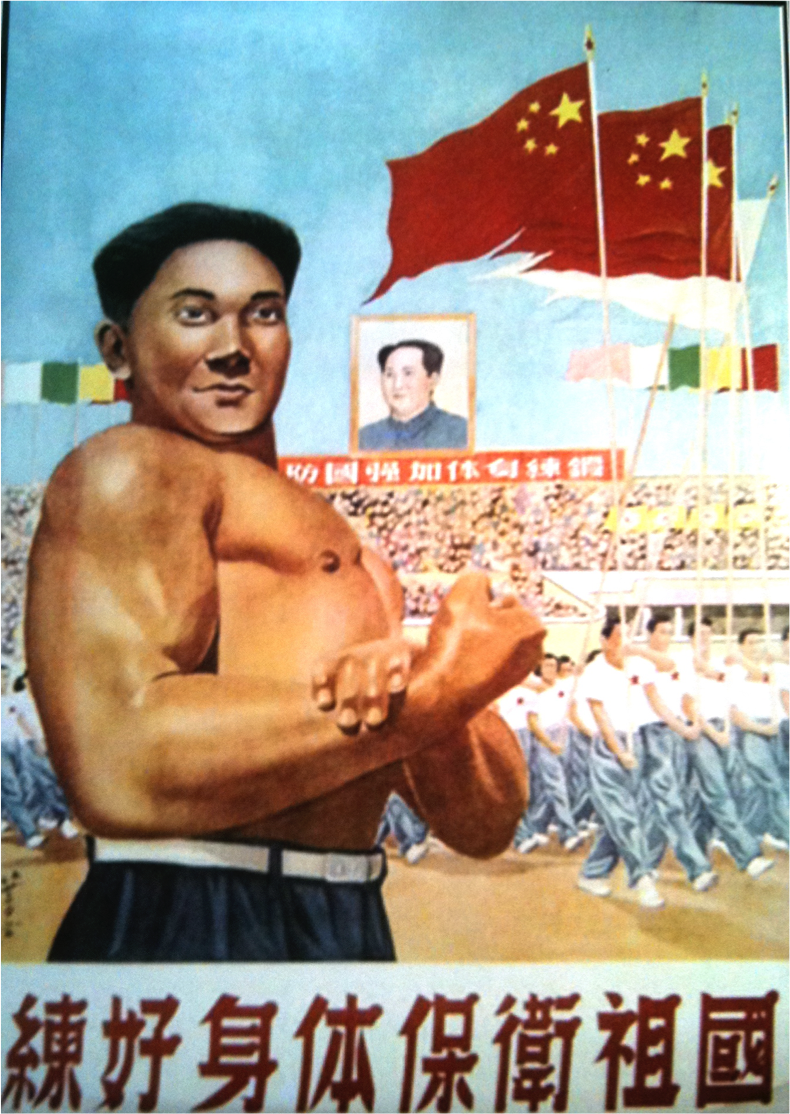
\includegraphics[width = \linewidth]{images/motherlandStrength.png}
  \caption{Strengthen Physique to Defend Motherland (1950)}
  \label{fig:motherlandStrength}
\end{figure}


The PRC Sport System
Along with many other facets of society after 1949, sport was institutionalised in line with Soviet bureaucratic models of governance.  In 1952 the ``State Sports (and Physical Culture) Commission'' (\textit{guojia tiyu yundon wieyuanhui} 国家体育运动委员会) (hereafter the Sports Commission) was established, which acted as the central State organ responsible for the administration of ``sport for the masses'' (\textit{qunzhong tiyu} 群众体育), ``physical culture education'' (\textit{tiyujiaoyu} 体育教育), as well as an elite competitive sport (\textit{jingji tiyu tixi} 竞技体育).


 In lieu of a sports system embedded within theThe competitive sport system was designed with the intention of creating a fast track for the development of world class athletic talent,


``tiyu for the masses'' and ``tiyu education'' by producing model athletes capable of performing and advocating the healthy, egalitarian and militaristic body promoted by the Party (Brownell 1995: 56).   The structure of the tiyu system exists today largely unchanged, although its name changed in 1998 to “The General Administration of Sport in China” (国家体育总局 Guojia tiyu zongju) (hereafter the Sports Administration).

%education programs for schools and other institutions)

At the bottom of the hierarchical structure are local sports commissions (county, township and city), above which are the provincial and municipal sports commissions; and at the top is the Sports Administration, located in Beijing (Brownell 1995: 59).  The Sports Administration is responsible for all sports training centres and sports programs, of which there are many types.  On one extreme there is the elite professional arm of the Sports Administration, a “national (tiyu) system” (juguo tizhi 举国体制), which
presides over all full-time professional sports teams (体工队 tigongdui) that exist at national and provincial/municipal levels.  The main objective of this national system is to cultivate elite athletes to compete on a national and international level, in events such as the National Games (全国运动会 Quanguo yundonghui), the Asian Games (亚洲运动会 Yazhou yundonghui), and most importantly, the Olympic games.  Due to an overwhelming Olympic-focus, all sports under the umbrella of professional arm of the Sports Commission are either Olympic sports, or Chinese martial arts (Guojia tiyu zongju 2009a).  Outside of this professional arm, elite tiyu programs are embedded within secondary and tertiary education institutions in a number of different ways, under the banner of the “high school and university tiyu system” (高校体制 gaoxiaotizhi) (Guojia tiyu zongju 2009a).  At a high school level, elite sports programs are offered at “extracurricular sports schools” (业余体校 yeyu tixiao), as well as regular high schools who focus on one or two tiyu programs in particular (Brownell 1995: 59). At a tertiary level, a number of specialist tiyu colleges operate at national, provincial/municipal and local levels.




The development of sport in China between 1949 - 1978 was hampered in many respects.  On the one hand, the internal political, social, and economic chaos of The Great Leap Forward (1955-58) and the Cultural Revolution (1966-77), detracted from a focus on development of sporting infrastructure and sporting development


as well as PRC's decision to boycott  from membership in the International Olympic Committee (IOC) and thus participation in the Olympic games, physical culture was nonetheless fundamental to the legitimacy of the PRC political regime (Xu 2008: 137).   The poster highlights the importance of the athlete in the Mao era as a key performer of the official culture of the body propagated by the party and directed at “the people” as an art of governance (Brownell 1995: 59).  As Brownell explains,
Mao linked the training of the body with the strength of the nation in a new way—through the notion of continuous revolution, which was to be carried out by an active body on behalf of a nation that was forever in motion (Brownell 1995: 57).
The co-option of “physical culture” as a governmental strategy, and its subsequent systematisation, served to instill an enduring logic of the body-and-nation in the hearts and minds of the Chinese population through the construction of a field—a world of sports in which understandings of the body and its use were contested and reproduced.





Reform era tiyu (1976-1988)
The death of Mao and the end of the Cultural Revolution in 1976 signalled the beginning of widespread social and economic transformations in China, in which the development of sport was heavily implicated.

Susan Brownell’s work, Training the Body for China (1995), the first and most comprehensive attempt at an anthropology of sport in China, was researched during the mid 1980s at a time when China was only just beginning to interact politically and economically with an international community.  In reference to the unprecedented success of the Chinese women’s volleyball team in the 1980s, including winning China's first ever gold medal in a team event at the LA Olympics in 1984, Brownell (1995: 86) explains how elite level sport functioned as a crucial symbolic practice for China in the process of ``rejoining the world.''  As a participant in the sports system as a student-athlete herself, Brownell draws on first-hand ethnographic experience of training and existing as subject to the state-administered ``microtechniques of power'' (citing Foucault 1977) designed to cultivate athletes in post-Mao China.  Brownell interrogates the role of the athlete in the perpetuation of a hyper-visible and generalisable moral order, cast in official terms as a ``socialist spiritual civilisation'' (jingshen wenming 精神文明) (1995: 156).  Brownell explains that the position of the athlete in reform era China was one characterised by the tensions and shifts of an ever-transforming social terrain structured by contradictory forces of the state and the emerging logic of the market.

One of the most immediate transformations to effect the Chinese sports system after the death of Mao was the restoration of the University Entrance Examination (gaokao 高考)
(hereafter gaokao), following the end of the Cultural Revolution in 1976 \citep[198]{Brownell1995}.  School curricula were immediately redesigned around the gaokao, and as a result, schools quickly reduced emphases on sport programs as they were seen to draw student’s attention and energy away from academic study.  A situation thus emerged where the only option for prospective athletes was to attend a specialist sports boarding school in which a scholastic education was not emphasised or was abandoned all together in favour of intense physical training.

Success on an international stage in the early 1980s delayed public scrutiny of this widening gap between education and sport. The The PRC won a total of 32 medals at the 1984 Los Angeles Olympics---its first official appearance at the Olympics since it boycotted the games in 1952 due to a dispute with the Republic of China (now Chinese Taipei) over the use of ``China.''  Importantly, 15 of these 32 medals were gold, and this powerful display of strength on the international stage was an enormous moment for modern Chinese nationalism in the reform era \citep{Brownell2008}.

When China produced a much less impressive performance in the summer Seoul Olympics in 1988, winning only 5 gold medals (and a total of 28), latent public criticism of way in which reform era sport had become isolated from society readily surfaced and a ``crisis in Chinese sports'' was declared \citep[199]{Brownell1995}.  Amidst broader social anxieties concerning not only the alarming quantity of the Chinese population (renkou guoduo 人口过多问题), but also the problem of population \textit{quality} (renkou suzhi 人口素质问题), the athlete in China was problematised as lacking sufficient ``cultural quality'' (wenhua suzhi 文化素质) in accordance with his or her elevated social status as a ``representative'' (daibiao 代表) of the Chinese nation on an ever-expanding international stage (General Administration of Sport 2009a; Brownell 1995: 95).

In response to this public sentiment, in 1988 former army general Wu Shaozu (伍绍祖) was
appointed head of national sports commission and tasked with implementing reform measures that would help the ``societization'' of the Chinese sport system. In 1989, for example, the Sports Commission adopted a policy modelled on the US college sports system, of ``combining sport and education'' (tijiao jiehe 体教结合).  In an attempt to move away from a reliance on sport boarding schools and full-time sports training centres for the development of athletic talent, ``high level tiyu programs'' (gaoji tiyu xiangmu 高级体育项目) were embedded within existing stand alone high schools and universities so as to ensure the ``all-round development''(quanmian fazhan 全面发展) of the athlete \citep[203]{Brownell1995}.  As part of an emphasis on a broader range of sports and their perceived potential to facilitate community engagement, international relations, as well as commercial opportunities, various sports programs, including many non-Olympic sports such as rugby, were inducted into the Chinese sports system for the first time\citep[70]{Knuttgen1990}.  Above all, the  democratisation of sports programs to include non-Olympic sports was driven by a persistent faith---built-in to the logic of ``physical culture'' form its inception int China---in the ability of sport to produce citizens of a certain \textit{quality} \citep[7]{Woronov2003}.


Reform measures continued into the mid 1990s. In an attempt to reduce the monopolisation of power and resources in the sports system, in 1993 Wu Shaozu broke up the six major sporting bodies of the Sports Commission into 23 sports management centres, with the ultimate goal of placing every sport under the management of an independent sporting association. In 1994 the first professional Chinese Football League was established, followed soon after by the professional Chinese Basketball League in 1995. In 1998, the Sports Commission rebranded as the General Administration of Sport (hereafter GAS) to accord with this direction of institutional reform.  But, one year earlier in 1997, powers above decided that Beijing would bid for the 2008 Olympics, and as such a subtle shift in focus occurred in Chinese sport that altered the course of reform.  Indeed, once the bid for the Olympics was announced as successful in 2001, sport reform ground to a halt as priority shifted to winning as many gold medals as possible \citep{News2017}.  Wu Shaozu left GAS in 2000, and his two successors Yuan Weimin (袁伟民, 2000-2004) Liu Peng
(刘鹏, 2004-2016) did not actively return to the project of reform, continuing to invest in Olympic performance.  Even though many sports had since established independent associations, these associations had to be directly affiliated with one of the 23 GAS has 23 sport management centres. Rugby, for example, was affiliated with the ``Management Centre for Small Ball Sports'' (小球管理中心),which was also home to sports such as golf and ten-pin bowling.

The lost decade:

Sport system became a space for scandal and corruption:

Public discontent concerning the persistence of China's narrow performance-focussed sports system was palpable throughout the 2000s.

CORRUPTION and SCANDAL:
marred by controversy:
corruption, match fixing etc
Doping reports


Yet, much like Groundhog Day, as was the case in the 1980s, these murmurings remained sufficiently muffled in public discourse by the strong performances of Chinese Olympic athlete delegations in Sydney 2000 (28 gold, 58 total) and Athens 2004 (32 gold, 63 total). The choreography of Chinese sporting might on the world stage reached its pinnacle when Beijing hosted the 2008 Olympics, with the Chinese athlete delegation winning 48 gold medals in a total haul of 100 medals.


"Low investment in public team sport, and deteriorating public health, contributed to lack of public participation, and the industry’s low value” (Wang Qi). CBA and CFA have suffered years of losses, not to mention table tennis and volleyball”

Many management centres have swelled into sovereign entities.

Power and money were concentrated in one pair of hands -vulnerable to corruption.  sports centres have moved away from We’s original reform goal, and become a hindrance to development of sports industry.


XI ERA REFORM:

Beijing 2022

Football:
Sport in 2015 announced as domestic consumption

Yao Ming

Table Tennis Coach dismissed.

Late 2016:  GZW blindisded sports centre managements, calling them monopolies and saying too much power rests in the hands of their chiefs.




%http://www.newschinamag.com/newschina/articleDetail.do?article_id=2409&section_id=15&magazine_id=22



\subsection{Rugby in China}
Although reportedly existing in China within colonial and expatriate circles for more than a century (Reason and Carwyn 1979: 210; HKRFU 2009), and as a modified military exercise as early as the 1930s (Morris 2004: 135), rugby was a late entrant into the Chinese sport system, established as a ``high level tiyu programs'' in 1990.  The advent of rugby in China can thus be understood in terms of the processes of tiyu “democratisation” explained above.  The introduction of rugby into China was initiated originally at CAU by professor Shi Zhengsheng (施振声) who was introduced to rugby by his supervising professor while completing vocational studies at Azabu University in Japan 1987-1989.  Following Shi’s return to CAU, an exchange relationship was set up between the two universities, and throughout 1990, coaches and referees from Azabu University came to CAU to help set up the necessary infrastructure required for a rugby program.  On the 12th December 1990, China’s first rugby union team was created.  The program was originally made up of existing CAU students who expressed interest in the novel activity, but by its second year, the program earned status as a “high level tiyu program” and was subsequently advertised to student-athletes across the country (Xu 2010: 2).  Between 1990 and 2010, rugby programs based on this original CAU model were established within over 30 regular universities and specialist sports colleges in cities throughout China.  There are also a number of social rugby clubs (俱乐部 julebu), organisations completely independent of the state sports system, in major cities with high expat populations (Shanghai, Beijing, Chengdu, Qingdao).


The Chinese Rugby Football Association (CRFA) was established in 1997. Both the men and women’s national teams, made up of players predominantly from CAU, but also from other well-established programs based at the Shanghai Sports University (沈阳体育学院 Shanghai tiyu xueyuan), Shenyang Sports College (沈阳体育学院 Shenyang tiyu xueyuan) and the People’s Liberation Army Sports College (中国人民解放军体育学院 Zhongguo renmin jiefangjun tiyu xueyuan), consistently compete against other nations in the Asia Pacific region (most notably in the Asian Games and the East Asian Games), and are also occasionally involved in top-tier international tournaments such as the International Hong Kong Sevens.

Before rugby became a professional sport in 2010, it had existed as a non-professional university sport for 20 years.  First established in 1990 at CAU, Beijing, rugby was and still is part of a large collection of ``cold-gate'' sports (\textit{lengmen xiangmu}, a term that refers to a profession, trade or branch of learning that receives little attention) in China, with a relatively small participation base compared to other interactive team sports like basketball or football.  While football and basketball have matured as standalone enterprises with supporting market-based consumer industries, most other sports in China (i.e., all other Olympic events, including rugby) exist primarily due to the support of the enormous state-sponsored sport system.  Whereas the commercial basketball and football industries might offer a small percentage of prospective athletes incentives of fame and fortune, the benefits of a state-sponsored sports programs like rugby are more modest.  Chinese youth either gravitate or are ushered by their parents towards sporting careers primarily due to potential life-course opportunities such as access to tertiary education and post-athletic career employment (in the government sports system).  The extent to which an athlete is able to maximise these potential benefits depends on the strength of an athlete's results (\textit{chengji}).
In Olympic sports, the most important measure of a province's success in state-sponsored sporting terms is the National Games, a quadrennial multi-sport event hosted on rotation by provincial capital cities \citep{Hong2002}.  The amount of funding a province and its provincial sporting institutes and programs receive is decided to a large extent by results at the national games.


However, due to the persistent Olympic focus of the Soviet-modelled Chinese competitive professional sports system (\textit{juguo tizhi}), rugby's recently acquired Olympic status means that it is one of 33 sports featured in the all important quadrennial National Games.  Ten of China's collection of 32 provinces and municipalities that participate in the National Games have full time men's and women's rugby programs.


When rugby union was inducted into the state sponsored sports system in 2010, a few Chinese provinces in particular identified a potential opportunity to achieve a beneficial National Games result by heavily investing in this debutant sport.  Beijing's Temple of Agriculture Sports Institute managed to attract a large amount of China's existing rugby talent—---including the unofficially touted ``Emperor'' (Boss) (\citep{huangdi}) of Chinese rugby, national coach Zheng Hongjun—--from where they were previously based at the Chinese Agricultural University, Beijing.  Meanwhile, Shandong province—--a powerhouse in other provincial sports--—succeeded in attracting the majority of the remaining talent, by token of the fact that a large majority of rugby players in China at the time (indeed, a large proportion of athletes more generally) were of Shandong origin.  Importantly, this talent included the Emperor's student come rival coach Lu Xiaohui.  Besides Beijing and Shandong, Jiangsu and Anhui province were strong contenders for the women's gold medal, while the People's Liberation Army (PLA) and Hong Kong in particular were strong contenders for top spot in the men's competition.

Beijing's results leading into the 2013 national games were strongest overall across the men's and women's teams, however the Hong Kong men's and women's teams had only occasionally participated in these tournaments.  In the semi-finals of the National Games, the Beijing men came up against Hong Kong, while the Shandong men played off against the PLA.  Beijing lost to their stronger and more favoured opponents, whereas Shandong beat the PLA.  Meanwhile in the women's league, both Beijing and Shandong advanced to the final.  The stage was set: Beijing, the favourites led by the reigning Emperor of Chinese rugby, would face Shandong, the underdogs lead by the Emperor's cunning apprentice.

The men's final was played first, and in somewhat of an upset, Shandong edged out Hong Kong to win the gold medal by one try.  In the women's final, scores were level until early in the 2nd half when Shandong went ahead by two tries to nil.  At that point, the Beijing women's team, under instruction from their coach Zheng Hongjun, suddenly stopped playing.  After being asked by the referee and match officials to continue, the Beijing women stood firm and refused to play on, forming a huddle on their side of half-way in the middle of the field. Shandong had no choice but to continue to play out the rest of the 2nd half, running in try after try, until the final score at full time was a farcical 71-0.  Shandong was declared victorious, while Beijing called foul play, claiming that the referee had been unfairly adjudicating the match in Shandong's favour.  The details and dramas of this now well-known story in China's sporting history (known as ``Match-striking-gate'') require more detailed development in a format that exists beyond the scope of this particular study. I introduce the story here in order to highlight its implications for my ethnographic research.

The Beijing women's rugby team was the first Beijing team in the 48-year history of the National Games not to receive the ``medal for civilised spirit''  (awarded by the Beijing Mayor to all Beijing representatives in the National Games) (SOURCE).  All rugby coaches and many senior athletes of the 2013 National Games campaign have since left the Temple of Agriculture: either retiring or moving to other provinces.  The rugby program was all but abandoned in 2014, and finally at the end of 2014 the men's program was resurrected by the appointment of a new head coach Zhu Peihou (a former Agricultural University Coach) and assistant Coach Shiyan.  The women's program was only formally re-established at the end of 2015, with the appointment of former Beijing women's rugby representative athlete Ma Jiale as head coach, and former Beijing men's rugby representative athlete Wang Chongyi as assistant coach.  Rugby is still part of the institute, but is no longer centre stage, and is a shadow of its former glory.  It was in this context that I entered the institute and conducted ethnographic research.














The second implication of this incident is what it says about the ethics of group membership in China.  This is not the first match-striking incident of Chinese sport. In fact, match-striking features periodically throughout recent Chinese sporting history.  In July 2015 Chinese ping pong athlete Zhang Weike failed to turn up to the 9th Round of the ping pong league because in protest at his club's refusal to sign a competition bonus agreement with him for that particular round of competition. The club were holding off signing the agreement because due to Zhang's recent poor form.  In 2004, Beijing Moderns Football Team famously stopped playing mid game against Shenyang Jinde Football Team due to objections with the referee's decisions. It was later revealed in an extensive expose of Chinese football in 2009 that the referee had in fact been bribed to fix the match (along with many other matches during that period), and this incident and many other like it were linked to the control of professional football in China by mafia-run betting rings.

The relevance of this incident to the present study is the fact that match-striking—--a strategy that appears to publicly disregard the sanctity of ``sporting contest''---exists as a viable strategy in the Chinese sporting world. That this option and others make up the behavioural arsenal of athletes, coaches, and officials in competitive sport in China is first an indication that sport in China suffers from a general lack of trust in the institutions that supposedly stand for values of fair play, sportsmanship, and the sporting contest; values often celebrated in Western democracies to be the foundational pillars of sport and worthy of fierce deontological defence in and of themselves\citep{Morris2004,Gold2002,Yuki2005}.
There have been various concerted attempts throughout China's modern history to instil the importance of ``fair play'' in Chinese sport \citep{Morris2004,Brownell1995,Brownell2008}, and yet, however intensely politicians, sports officials, coaches, and athletes emphasise in official public rhetoric the importance of such categorical ideals in sport, it is also clear that the behaviour of these very same agents is often heavily determined by networks of power (\textit{quanli}) and interest (\textit{liyi}) that function externally to official institutions and threaten the exact values that are publicly promoted.

%%%%%
China's modern history has been turbulent, tragic, and continually in flux, and sport forms part of this greater story.  While a full dealing with sport in China is beyond the parameters of this dissertation, it is interesting to note that, from a cultural-psychological perspective, interactive team sports in particular have proven far from a ``snug fit'' for China.  Save for occasional flashes of glory in women's volleyball (Gold Medalists at Los Angeles Olympics in 1980), China's team sports have traditionally underperformed on the International stage, to the great embarrassment of the nation \citep{Brownell2008}.  This national embarrassment is most intensely felt in relation to the Chinese men's football team, who often record defeats to minnow neighbouring countries such as Thailand and Hong Kong. When asking my research subjects about the China's team sport issue, a series of physiological and psychological reductions are offered for Chinese peoples' deficiency in the cooperation requirements of team sports: China's one child policy, a culturally-instituted deference to authority and lack of creativity, and a conviction that that Chinese society is too complex and Machiavellian to support pure commitment to the team.  How is it possible to assess these discursive explanations in light of cognitive and evolutionary mechanisms of cultural transmission and social cohesion?

The extent to which cultural psychological processes support and help reproduce the specific socio-ecological phenomenon of sport in contemporary China should also be carefully considered \citep{Sperber1996,Nisbett2003}.  On this level of analysis, the prevalence of scandal and corruption in Chinese sport is perhaps symptomatic of a complex ecology of cultural practices structured by both relational and categorical psychological tendencies relating to social interaction, group formation, and cultural institutions \citep{Nisbett2003,Yuki2005,Liu2009}.\footnote{Indeed, the naivety with which Western countries appear to maintain faith in the sanctity of sport as a pure space for the cultivation and display of virtue and mutual respect, despite obvious evidence to the contrary (use of performance enhancing drugs, match-fixing scandals, exploitation of athletes, etc.) should also be called into question \citep{Southall2017}.  Unfortunately a proper investigation of these questions lie outside the bounds of this dissertation.} What makes group exercise so fascinating is the way in which the culturally-specific patterns and signatures of these complex psychosocial processes can be witnessed at once in the most macro-scale of institutional organisation, right through to the most subtle movement tendency in joint action on the field.


%It is important to approach a study of joint action and social bonding between Chinese professional rugby players with this cultural-psychological variation in mind.
%While the cognitive processes of joint action and social may exist as hypothesised, they may come packaged in  discourses and behavioural tendencies shaped by the specific cultural context.


\subsection{Joint action, team click, and social bonding in China}
As mentioned above, while there is very little empirical evidence linking movement coordination and social bonding within the Chinese cultural context, there is extensive indirect evidence from historical and contemporary literatures to suggest ways in which this relationship---between (joint) action and social processes of group formation and cohesion---is uniquely articulated in the Chinese context \citep{Weed2011}.  Historical evidence also suggests that the dynamics of joint action in particular have the focus of ethical considerations, namely resolution of social tensions inherent in collective action problems \citep{Slingerland2014}.

It is well documented that the most prominent metaphor in Chinese cultural discourse is that of the family \citep{Maehr1980}, and that this metaphor structures many extra-kin social relationships between individuals, and between the individual and the state \citep{Gold2002}.  Traditionally, the father-son kinship relationship is utilised to naturalise the socially constructed relationship between lord and minister: ``Parents naturally love their children, and children naturally love and respect their parents, and they both know that they're stuck with one another no matter what...'' \citep[178]{Slingerland2014}. Likewise, the metaphor of family is often utilised to naturalise the notion of an extra-kin social group, for example a company or a sporting team \citep{Brownell2008}.
It is important to emphasise that, whereas traditionally Western (Anglo-American) notions of group membership generally hinge upon a psychological representation of egalitarian equivalence between categories of self and group, the utilisation of the family metaphor for group processes relies on the individual identifying group membership through a participation in hierarchically structured (familial-like) \textit{relationships} \citep{Fei1992}.

It is within these processes of extending familial metaphors to formal social relationships that Slingerland (2014) locates a key role for joint action. Inherent in the scaling up of familial relationships to extra-kin social relationships is the tension common to many collective action problems, that of vulnerability to free-riding and defection \citep{Cosmides2013,Gavrilets2015}.
As Slingerland explains, the ``logic of civilised life makes us very keen to distinguish reliable cooperators from unreliable defectors...what we want then is a particular type of desirable...behaviour where there is absolutely no gap between action and motivation'' \citep[192]{Slingerland2014}. The paradoxical Chinese idiom of \textit{wei wuwei}, translated awkwardly into English as ``trying not to try'' or ``effortless action,'' is promoted in many ancient Chinese philosophical corpuses as a behavioural solution to conflicting incentives involved in coordination problems: effortlessness in performing socially desirable actions (virtues) communicates a level of mutual trust and commitment that is ``hard-to-fake.''  The phenomenology of effortless action is described at length in many of these corpuses, and is a key dimension of many traditional Chinese martial arts such as Taichi and Wushu \citep{Morris1998}.
While mass participation in Anglo-American competitive sports is only a recent phenomenon in China \citep{Brownell2008}, the social valorisation of certain types and styles of movement, particularly the phenomenology of flow in (joint) action appears to enjoy a long history.


\subsection{Modes of group membership and self-construal}
An analysis of literature concerning the cultural psychology of self-construal can provide important insights into the way in which macro cultural processes interact with micro-dynamics of social interaction to structure and constrain cognitive processes implicated with joint action, team click, and social bonding.  As Anthropologists have emphasised for some time \citep{Strodtbeck1961,Kluckhohn1961,Mead1967,Fei1992}, and as cultural psychologists are now beginning to demonstrate in experimental paradigms, processes of group membership appear to vary cross-culturally \citep{Markus1991,Nisbett2001}.  Based on recent cross-cultural research, social and cultural psychologists have developed a theoretical spectrum of group membership processes, the two poles of which can be described as categorical and relational \citep{Hofstede1980,Brewer2007}.  Whereas some cultures, traditionally ``Western'' cultures such as the US, the core of self-definition is based on individual autonomy and separation from others.
The self-concept of relational societies, traditionally understood to be predominantly East Asian cultures, by contrast, is defined primarily based on social embeddedness and interdependence with others comprising their in-groups\citep{Leung2012}.

Unsurprisingly, much of Anglo-American social psychology of the 20th Century is rooted in a categorical mode of representing and measuring group membership.  The canonical self-categorisation paradigm of social psychology \citep{Turner1987}, for example, requires that a bounded individual (experimental subject) make an identification between abstract categories of the self and the in-group or out-group.  Categorical group membership is thus achieved when the perceived differences between the self and other in-group members are smaller than the differences between in-group and out-group members \citep{Yuki2014}.  In distinction to a categorical mode of group membership, relational group membership involves attention to maintaining and harmonising intragroup relationships, engaging in intergroup categorical comparisons \citep{Yuki2003}.
In a relational mode, social identity is less a function of distance between abstract categories of self and in-group, and more a degree of commitment to cultivating a network of hierarchically structured---but more or less self-centred and self-enhancing---network of relationships \citep{Liu2009,Nisbett2003}.

These two predominant modes of group membership—--categorical and relational—--have been shown to vary across cultures (i.e. East Asian versus Western European or North American, see \citep{Markus1991,Nisbett2001,Yuki2003}, within groups (according to sex and personality differences \citep{Yuki2014}, and indeed, within individuals (depending on contextual and situational primes, \citep{Lee2014,Wong2005}).  While the durable persistence of cultural and linguistic institutions appear to be responsible for the prominence of one mode of membership over another (East versus West, for example), recently researchers have suggested that divergent modes of group membership—categorical and relational—may be mediated by context-specific socio-ecological factors such as the level of relational mobility in any given environment \citep{Oishi2010,Takagishi2014,Yuki2005}.  Both modes of group membership have been shown to shape attention, cognition, and behaviour \citep{Nisbett2003} and as such have important implications for the task of identifying and measuring social bonding mechanisms of joint action

Experimental evidence suggests that categorical group processes facilitate fast and effective identification with arbitrary minimal groups \citep{Diehl1990,VanBavel2014}, the arousal of intrapersonal cognitive dissonance between the self and experimentally constructed in-group \citep{Festinger1957, Stone2001}, higher levels of cooperation with categorically similar strangers in economic games \citep{Yuki2005,Yuki2003}, and greater attention to and memory recall \citep{Buchan2006,Ng2016}.  In cultural environments where relational processes of group membership are more prominent or salient, on the other hand, the inverse is usually observed. First, minimal group paradigms have had very little (if any) success in East Asian (particularly Japanese) contexts \citep{Liu2009}.  Relational group processes, on the other hand, allow for the arousal of cognitive dissonance only when it is constructed interpersonally (as opposed to intrapersonally) between an individual and specific individuals to which that individual is connected by a meaningful social relationships \citep{Hoshino-Browne2005}.  Likewise, individuals with a predominantly relational group awareness are more willing to cooperate with and attend to strangers with whom they share relational rather than categorical ties \citep{Ng2016,Yuki2005}.

Relational group membership has a long history in China, rooted in Confucian \citep{Hwang1999}, folk-cultural axioms \citep{Wang2009}, agricultural modes of production \citep{Talhelm2014,Fei1992}, dynastic rule, and modern reinventions of these cultural forms by processes of the nation-state\citep{Liu2014}. The metaphor of the family is particularly salient and pervasive in modern public representations.  On almost every scale of social organisation, from dyadic extra-kin friendships through to workplace interactions and macro-social organisations (cities, provinces, nation), the family and its relational priorities are consistently invoked to aid coordination and coerce participation in collection action.
In addition, the last 150 years of Chinese modern history has also entailed the introduction of categorical group processes associated with the activities of the nation-state, leading to a contemporary Chinese indigenous psychology in which a relational mode is predominant, and a categorical mode is contextually-activated, especially when categories such as ``China'' are threatened or challenged internationally \citep{Liu2009}.

\subsection{Implications for the present study}
The literature reviewed above potentially poses an interesting challenge to the way in which social bonding is understood within cognitive and evolutionary anthropology.  The professional Chinese rugby players that form the focus of this dissertation are young men and women predominantly from rural areas of China's northeast, and are therefore likely subject to relational modes of group membership made predominant and durable by persistent cultural and linguistic processes associated with group membership in contemporary China \citep{Liu2009}.  In addition, athletes are members of a relatively small and stable team environment, for which access to benefits should require attention to the maintenance of productive intragroup relationships, more so than processes of intergroup mobility or comparison \citep{Schug2010}, even though intergroup comparison is an inherent component of competitive interactional team sport. However, given the fact that rugby is an imported team-based interactive sport, for which categorical modes of group membership are required and celebrated, I also expect athletes to exhibit a categorical mode of group membership.
In addition, I expect the metaphors of family to be prominent in the scaffolding of team processes, and I also expect to find a tension between loyalties to the team, and loyalties to an athlete's pre-existing relational networks of family and friends\citep{Yang1994}.  Thus, the specific cultural setting is such that I do not necessarily expect to encounter the type of public representation or testimony of group membership common in Western sporting parlance, more indigenous to the rugby pitches and boathouses of Oxford or any high school American Football movie produced in the 1990s.  Instead, I expect to find evidence of a link between joint action, team click, and social bonding expressed and embodied in cultural representations that may vary distinctly in structure and content from Western intuitions based on a predominantly categorical mode of social cognition.





%In 1820, China's urban population began to grow from a low of 6\% approximately 90\% of China's population of 243 million lived in small rural village organisation \citep{Zheng2005}), and this number increased to

243 million in 1778

This basic economic tension in trade relations between Britain and China fueled the

 which was initiated by the British Empire throughand then

Treaty of Nanking 1842

marked by the devastating Opium wars (1 First Opium War (1839–1842) ) left China's intellectual elite to seek the regeneration of China in the form of a modern nation state.
